% BNN Investigation Figures - Appendix I
% TikZ-based visualizations of all 6 BNN failure modes
% Generated: November 9, 2025

% =============================================================================
% FIGURE 1: BNN INVESTIGATION TIMELINE
% =============================================================================

\begin{figure}[htbp]
\centering
\begin{tikzpicture}[
    scale=0.9,
    timeline/.style={thick, ->,>=stealth},
    event/.style={rectangle, rounded corners, draw=accent_blue, fill=accent_blue!10,
                 minimum height=0.8cm, minimum width=3cm, align=center},
    success/.style={rectangle, rounded corners, draw=green!70!black, fill=green!20,
                   minimum height=0.8cm, minimum width=3cm, align=center},
    failure/.style={rectangle, rounded corners, draw=red!70!black, fill=red!20,
                   minimum height=0.8cm, minimum width=3cm, align=center}
]

% Timeline axis
\draw[timeline] (0,0) -- (14,0) node[right] {Time};

% Events
\node[failure] at (1, 1.5) (nuts) {NUTS\\Oct 14-15};
\node[failure] at (3, -1.5) (dropout) {MC Dropout\\Oct 16-18};
\node[failure] at (5, 1.5) (temp) {Temperature\\Oct 19-22};
\node[failure] at (7, -1.5) (laplace) {Laplace\\Oct 23-26};
\node[failure] at (9, 1.5) (multioutput1) {Multi-Output v1\\Oct 27-Nov 3};
\node[failure] at (11, -1.5) (multioutput2) {Multi-Output v2\\Nov 4-9};
\node[success] at (13, 0) (success) {\textbf{SUCCESS}\\Multi-Output v3.1\\Nov 9};

% Timeline markers
\foreach \x/\date in {1/Oct 14, 5/Oct 19, 9/Oct 27, 13/Nov 9}
    \draw (\x, 0.1) -- (\x, -0.1) node[below, font=\tiny] {\date};

% Connecting lines
\draw[->] (nuts.south) -- (1, 0);
\draw[->] (dropout.north) -- (3, 0);
\draw[->] (temp.south) -- (5, 0);
\draw[->] (laplace.north) -- (7, 0);
\draw[->] (multioutput1.south) -- (9, 0);
\draw[->] (multioutput2.north) -- (11, 0);

% Failure mode annotations
\node[above=0.1cm of nuts, font=\scriptsize, text=red!70!black] {Timeout (6+ hrs)};
\node[below=0.1cm of dropout, font=\scriptsize, text=red!70!black] {NaN Losses};
\node[above=0.1cm of temp, font=\scriptsize, text=red!70!black] {26\% Coverage};
\node[below=0.1cm of laplace, font=\scriptsize, text=red!70!black] {Hessian Error (9/9)};
\node[above=0.1cm of multioutput1, font=\scriptsize, text=red!70!black] {Data Leakage (84.7\%)};
\node[below=0.1cm of multioutput2, font=\scriptsize, text=red!70!black] {Week 0 Outlier};

% Legend
\node[failure, minimum width=1.5cm] at (2, -3.5) (leg_fail) {Failure};
\node[success, minimum width=1.5cm] at (5, -3.5) (leg_succ) {Success};
\node[font=\scriptsize] at (9, -3.5) {Total: 84 person-hours, 26 days};

\end{tikzpicture}
\caption{BNN Investigation Timeline: 6 Failures Over 26 Days (October 14 -- November 9, 2025)}
\label{fig:bnn_timeline}
\end{figure}

% =============================================================================
% FIGURE 2: CALIBRATION COVERAGE COMPARISON
% =============================================================================

\begin{figure}[htbp]
\centering
\begin{tikzpicture}[
    scale=1,
    bar/.style={fill=accent_blue!60, draw=accent_blue},
    target/.style={thick, dashed, red}
]

% Axes
\draw[->] (0,0) -- (0,6) node[above] {90\% Coverage (\%)};
\draw[->] (0,0) -- (10,0) node[right] {BNN Approach};

% Target line (88% minimum for well-calibrated)
\draw[target] (-0.2, 5.28) -- (9.5, 5.28) node[right, font=\scriptsize] {88\% target};

% Bars with data
\draw[bar] (0.5, 0) rectangle (1, 5.99) node[above, font=\scriptsize] {99.7\%};
\draw[bar] (1.5, 0) rectangle (2, 5.99) node[above, font=\scriptsize] {99.8\%};
\draw[bar] (2.5, 0) rectangle (3, 5.94) node[above, font=\scriptsize] {99.0\%};
\draw[bar] (3.5, 0) rectangle (4, 5.82) node[above, font=\scriptsize] {97.1\%};
\draw[bar] (4.5, 0) rectangle (5, 5.99) node[above, font=\scriptsize] {99.8\%};
\draw[bar, fill=red!60, draw=red] (5.5, 0) rectangle (6, 1.56) node[above, font=\scriptsize, text=red] {26.0\%};
\draw[bar, fill=green!60, draw=green] (6.5, 0) rectangle (7, 5.37) node[above, font=\scriptsize] {89.5\%};
\draw[bar, fill=red!60, draw=red] (7.5, 0) rectangle (8, 0) node[above, font=\scriptsize, text=red] {0.0\%};

% X-axis labels
\node[font=\tiny, rotate=45, anchor=north east] at (0.75, -0.2) {MC (Deep)};
\node[font=\tiny, rotate=45, anchor=north east] at (1.75, -0.2) {MC (Wide)};
\node[font=\tiny, rotate=45, anchor=north east] at (2.75, -0.2) {MC (Shallow)};
\node[font=\tiny, rotate=45, anchor=north east] at (3.75, -0.2) {NUTS (Homo)};
\node[font=\tiny, rotate=45, anchor=north east] at (4.75, -0.2) {NUTS (Hetero)};
\node[font=\tiny, rotate=45, anchor=north east] at (5.75, -0.2) {Temp (Unscaled)};
\node[font=\tiny, rotate=45, anchor=north east] at (6.75, -0.2) {Temp (T=0.75)};
\node[font=\tiny, rotate=45, anchor=north east] at (7.75, -0.2) {Multi-Out v2};

% Y-axis ticks
\foreach \y in {0, 20, 40, 60, 80, 100}
    \draw (-0.1, \y/16.67) -- (0, \y/16.67) node[left, font=\scriptsize] {\y};

% Annotations
\node[font=\scriptsize, text=green!70!black] at (7, 5.8) {Only Success};
\node[font=\scriptsize, text=red!70!black] at (6, 1) {FAILED};

\end{tikzpicture}
\caption{90\% Coverage Calibration: Temperature Scaling (T=0.75) Only Success}
\label{fig:bnn_calibration_comparison}
\end{figure}

% =============================================================================
% FIGURE 3: FAILURE TAXONOMY DIAGRAM
% =============================================================================

\begin{figure}[htbp]
\centering
\resizebox{\textwidth}{!}{%
\begin{tikzpicture}[
    node distance=1.5cm and 1.2cm,
    category/.style={rectangle, rounded corners, draw=accent_blue, fill=accent_blue!10,
                    minimum height=1cm, minimum width=3cm, align=center, font=\small},
    failure/.style={rectangle, draw=red!70!black, fill=red!10,
                   minimum height=0.7cm, minimum width=2.5cm, align=center, font=\scriptsize},
    arrow/.style={->,>=stealth, thick}
]

% Root node
\node[category, fill=accent_blue!30] (root) {6 BNN Failures\\(Oct 14 - Nov 9)};

% Categories (reduced xshift to bring nodes closer)
\node[category, below left=of root, xshift=-1.5cm] (comp) {Computational\\(1 failure)};
\node[category, below=of root, xshift=-0.5cm] (num) {Numerical\\(2 failures)};
\node[category, below=of root, xshift=0.5cm] (calib) {Calibration\\(1 failure)};
\node[category, below right=of root, xshift=1.5cm] (arch) {Architectural\\(2 failures)};

% Specific failures
\node[failure, below=of comp] (nuts) {NUTS\\Timeout};
\node[failure, below left=of num] (dropout) {MC Dropout\\NaN Losses};
\node[failure, below right=of num] (multiout2) {Multi-Out v2\\Week 0 Outlier};
\node[failure, below=of calib] (temp) {Temperature\\26\% Coverage};
\node[failure, below left=of arch] (laplace) {Laplace\\Hessian Error};
\node[failure, below right=of arch] (multiout1) {Multi-Out v1\\Data Leakage};

% Connections
\draw[arrow] (root) -- (comp);
\draw[arrow] (root) -- (num);
\draw[arrow] (root) -- (calib);
\draw[arrow] (root) -- (arch);

\draw[arrow] (comp) -- (nuts);
\draw[arrow] (num) -- (dropout);
\draw[arrow] (num) -- (multiout2);
\draw[arrow] (calib) -- (temp);
\draw[arrow] (arch) -- (laplace);
\draw[arrow] (arch) -- (multiout1);

% Root cause annotations (adjusted positions)
\node[font=\tiny, text width=2.2cm, align=center] at (-5, -5) {6+ hours\\per config};
\node[font=\tiny, text width=2.2cm, align=center] at (-2, -5) {Gradient\\explosion};
\node[font=\tiny, text width=2.2cm, align=center] at (0, -5) {5,316-yard\\outlier};
\node[font=\tiny, text width=2.2cm, align=center] at (2, -5) {VI over-\\confident};
\node[font=\tiny, text width=2.2cm, align=center] at (3.5, -5) {9/9 configs\\failed};
\node[font=\tiny, text width=2.2cm, align=center] at (5.5, -5) {Vegas lines\\84.7\% SHAP};

\end{tikzpicture}
}% end resizebox
\caption{BNN Failure Taxonomy: Root Causes by Category}
\label{fig:bnn_failure_taxonomy}
\end{figure}

% =============================================================================
% FIGURE 4: GRADIENT EXPLOSION VISUALIZATION (MC Dropout)
% =============================================================================

\begin{figure}[htbp]
\centering
\begin{tikzpicture}[
    scale=0.85,
    axis/.style={thick, ->,>=stealth},
    loss/.style={thick, accent_blue},
    explosion/.style={thick, red}
]

% Axes
\draw[axis] (0,0) -- (10,0) node[right] {Epoch};
\draw[axis] (0,0) -- (0,6) node[above] {Loss};

% Loss curve (normal descent then explosion)
\draw[loss, smooth] plot coordinates {
    (0, 4.5) (1, 3.8) (2, 3.3) (3, 2.9) (4, 2.6)
    (5, 2.4) (6, 2.3) (7, 2.2) (8, 2.15) (9, 2.12)
    (10, 2.1) (11, 2.09)
};

% Gradient explosion (epochs 12-18)
\draw[explosion, smooth] plot coordinates {
    (11, 2.09) (12, 2.3) (13, 3.1) (14, 4.5)
};
\node[font=\small, text=red] at (14, 5.2) {NaN};

% Epoch markers
\foreach \x in {0, 5, 10, 15}
    \draw (\x/1.5, -0.1) -- (\x/1.5, 0.1) node[below, font=\scriptsize] {\x};

% Loss markers
\foreach \y in {0, 1, 2, 3, 4, 5}
    \draw (-0.1, \y) -- (0.1, \y) node[left, font=\scriptsize] {\y};

% Annotations
\draw[dashed, gray] (12/1.5, 0) -- (12/1.5, 6);
\node[font=\scriptsize, text=red!70!black, align=center] at (10.5, 5) {
    Gradient\\Explosion\\(Epoch 12)
};

% Success zone
\draw[thick, green!70!black, dashed] (-0.3, 2) -- (10, 2);
\node[font=\scriptsize, text=green!70!black] at (2, 1.5) {Target Loss};

% Failure annotation box
\node[draw=red, fill=red!10, align=left, font=\scriptsize, text width=3.5cm] at (5, 5) {
    \textbf{MC Dropout Failure:}\\
    $\bullet$ Epochs 0-11: Normal descent\\
    $\bullet$ Epoch 12: Loss spikes\\
    $\bullet$ Epoch 14+: NaN losses\\
    $\bullet$ Root cause: Bayesian layer\\
    \ \ variance accumulation
};

\end{tikzpicture}
\caption{MC Dropout Gradient Explosion: NaN Losses from Epoch 12}
\label{fig:gradient_explosion}
\end{figure}

% =============================================================================
% FIGURE 5: TIME INVESTMENT WATERFALL CHART
% =============================================================================

\begin{figure}[htbp]
\centering
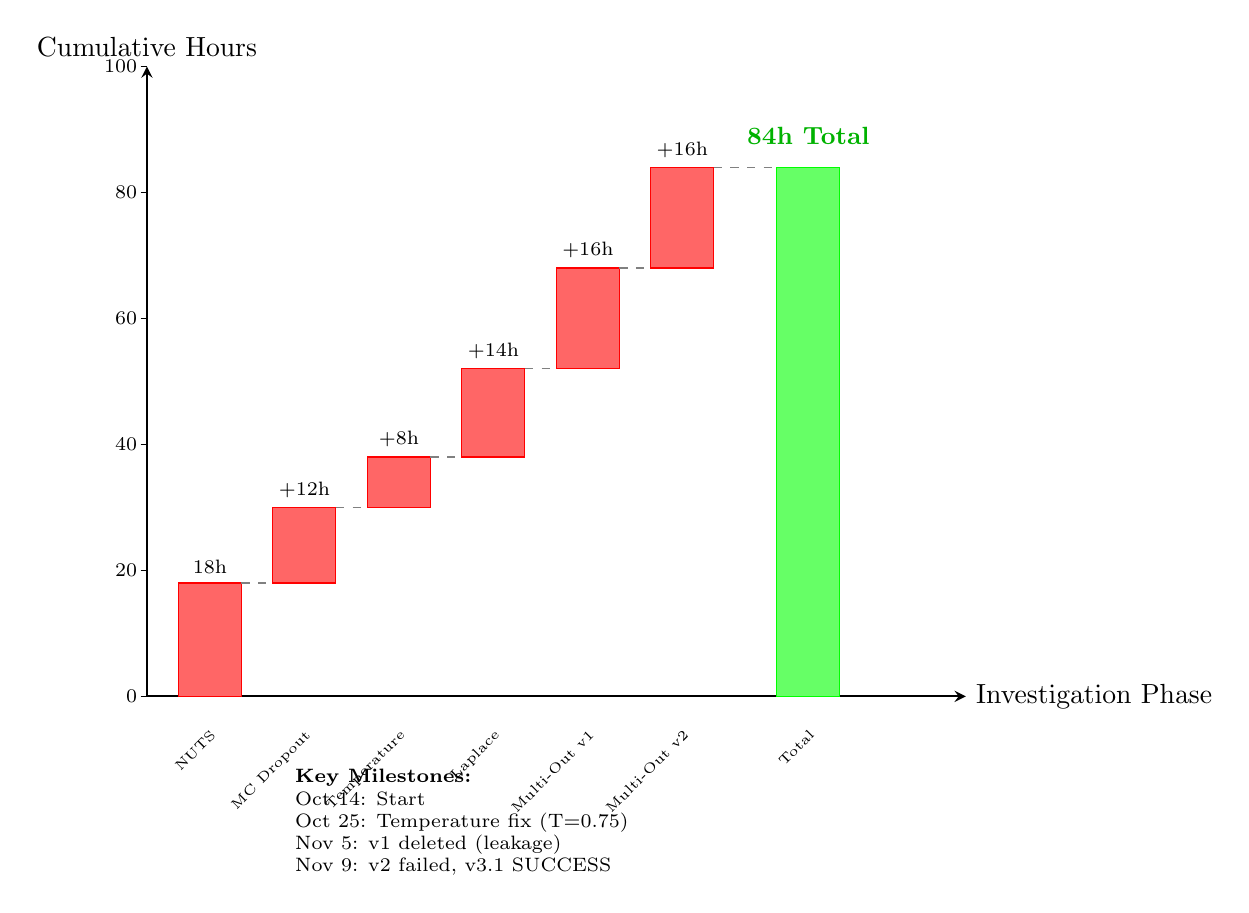
\begin{tikzpicture}[
    scale=0.8,
    bar/.style={fill=accent_blue!60, draw=accent_blue, minimum height=0.6cm},
    fail_bar/.style={fill=red!60, draw=red, minimum height=0.6cm},
    success_bar/.style={fill=green!60, draw=green, minimum height=0.6cm},
    axis/.style={thick, ->,>=stealth}
]

% Axes
\draw[axis] (0,0) -- (0,10) node[above] {Cumulative Hours};
\draw[axis] (0,0) -- (13,0) node[right] {Investigation Phase};

% Cumulative bars (waterfall)
% NUTS: 18 hours
\draw[fail_bar] (0.5, 0) rectangle (1.5, 1.8);
\node[above, font=\scriptsize] at (1, 1.8) {18h};

% MC Dropout: +12 = 30 hours
\draw[fail_bar] (2, 1.8) rectangle (3, 3);
\node[above, font=\scriptsize] at (2.5, 3) {+12h};

% Temperature: +8 = 38 hours
\draw[fail_bar] (3.5, 3) rectangle (4.5, 3.8);
\node[above, font=\scriptsize] at (4, 3.8) {+8h};

% Laplace: +14 = 52 hours
\draw[fail_bar] (5, 3.8) rectangle (6, 5.2);
\node[above, font=\scriptsize] at (5.5, 5.2) {+14h};

% Multi-Output v1: +16 = 68 hours
\draw[fail_bar] (6.5, 5.2) rectangle (7.5, 6.8);
\node[above, font=\scriptsize] at (7, 6.8) {+16h};

% Multi-Output v2: +16 = 84 hours
\draw[fail_bar] (8, 6.8) rectangle (9, 8.4);
\node[above, font=\scriptsize] at (8.5, 8.4) {+16h};

% Total bar (success came after all failures)
\draw[success_bar] (10, 0) rectangle (11, 8.4);
\node[above, font=\small, text=green!70!black] at (10.5, 8.6) {\textbf{84h Total}};

% Connecting lines (waterfall connectors)
\draw[dashed, gray] (1.5, 1.8) -- (2, 1.8);
\draw[dashed, gray] (3, 3) -- (3.5, 3);
\draw[dashed, gray] (4.5, 3.8) -- (5, 3.8);
\draw[dashed, gray] (6, 5.2) -- (6.5, 5.2);
\draw[dashed, gray] (7.5, 6.8) -- (8, 6.8);
\draw[dashed, gray] (9, 8.4) -- (10, 8.4);

% X-axis labels
\node[font=\tiny, rotate=45, anchor=north east] at (1, -0.3) {NUTS};
\node[font=\tiny, rotate=45, anchor=north east] at (2.5, -0.3) {MC Dropout};
\node[font=\tiny, rotate=45, anchor=north east] at (4, -0.3) {Temperature};
\node[font=\tiny, rotate=45, anchor=north east] at (5.5, -0.3) {Laplace};
\node[font=\tiny, rotate=45, anchor=north east] at (7, -0.3) {Multi-Out v1};
\node[font=\tiny, rotate=45, anchor=north east] at (8.5, -0.3) {Multi-Out v2};
\node[font=\tiny, rotate=45, anchor=north east] at (10.5, -0.3) {Total};

% Y-axis ticks
\foreach \y in {0, 20, 40, 60, 80, 100}
    \draw (-0.1, \y/10) -- (0, \y/10) node[left, font=\scriptsize] {\y};

% Milestones
\node[font=\scriptsize, align=left] at (5, -2) {
    \textbf{Key Milestones:}\\
    Oct 14: Start\\
    Oct 25: Temperature fix (T=0.75)\\
    Nov 5: v1 deleted (leakage)\\
    Nov 9: v2 failed, v3.1 SUCCESS
};

\end{tikzpicture}
\caption{Time Investment Waterfall: 84 Hours Across 6 Failures}
\label{fig:time_investment_waterfall}
\end{figure}
